\documentclass[10pt,conference,compsocconf]{IEEEtran}

\usepackage{hyperref}
\usepackage{graphicx}	% For figure environment

\begin{document}
\title{Class Project 1}

\author{%
  Saskia Reiss, Alvaro Pinedo and David Resin\\%
  CS-433 -- Machine Learning\\EPFL, Switzerland%
}

\maketitle

\begin{abstract}
Machine learning is for many the future of computer science and in the wider sense the future of science. Indeed there is barely any field of expertise where we are not faced with huge abstract datasets that contain the key to our problem. One of these fields is quantum physics and the attempts at widening the standard model of particle physics. One milestone in these attempts was in 2013, when researchers at the LHC managed to prove the existence of the Higgs boson, which is responsible for the existence of mass, which was predicted by Peter Higgs half a century earlier. This achievement could not have been possible without machine learning, and its power to make sense of the huge amounts of data generated by high-energy proton-proton collisions. Here we will attempt to reproduce this by working on a genuine dataset from the LHC.
\end{abstract}
\section{Introduction}
This work will consist of an application of various methods seen in lectures as well as work of our own to try and get the best estimation possible from a provided dataset of thousands of samples of 30 different parameters to attempt to predict whether each sample is a Higgs boson or not.
\begin{figure}[h!]
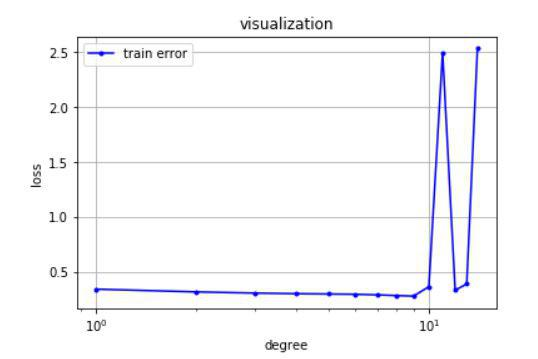
\includegraphics[width=.5\textwidth]{losses_least_squares.jpg}
\caption{Losses for different degrees for \texttt{least\_squares}}
\end{figure}
\section{Methodology}
First, we extract the data from the \texttt{.csv} files using the provided function \texttt{load\_csv\_data}. For each file it returns us the predictions \texttt{y} (which is of course empty in the case of the test data), the data \texttt{x}, and the sample identifiers \texttt{ids}. We defined the function \texttt{triage} which replaces all $-999$ values in the document, which are placeholders for unavailable data, with the mean of the column they are in. We consider this to be the best way to treat these values without splitting up the data into different categories. We decided not to normalize the data as it resulted in overfitting. We then use the \texttt{build\_poly} method with degree 9 on both datasets, before applying \texttt{least\_squares} on the training data set and feed the resulting weigths to \texttt{predict\_labels} along with the testing dataset.

\section{Results}
\begin{itemize}
\item Our first attempt simply used \texttt{least\_squares} on the unaltered dataset, which gave us a score of \textbf{0.74463}.
\item We then improved our results by applying \texttt{build\_poly} with degree 7 and feeding the result to \texttt{least\_squares}, which gave us a new best score of \textbf{0.80061}.
\item Our next improvement  consisted of replacing all $-999$ values in the dataset with 0's instead for a score of \textbf{0.80596}.
\item Ridge regression with lambda worth $2.6826957952797275 \cdot 10^{-9}$ gave us a score of \textbf{0.81549}.
\item Replacing $-999$ values with the column average instead along with building polys of degree 9 raised our best score to \textbf{0.81553}.
\end{itemize}
\begin{figure}[h!]
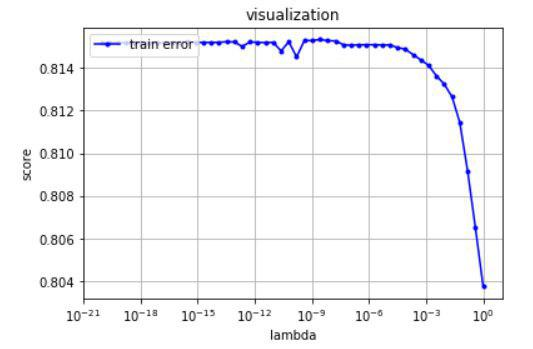
\includegraphics[width=.5\textwidth]{ridge_reg_scores.jpg}
\caption{The scores for different lambdas for our ridge regression}
\end{figure}
\begin{figure}[h!]
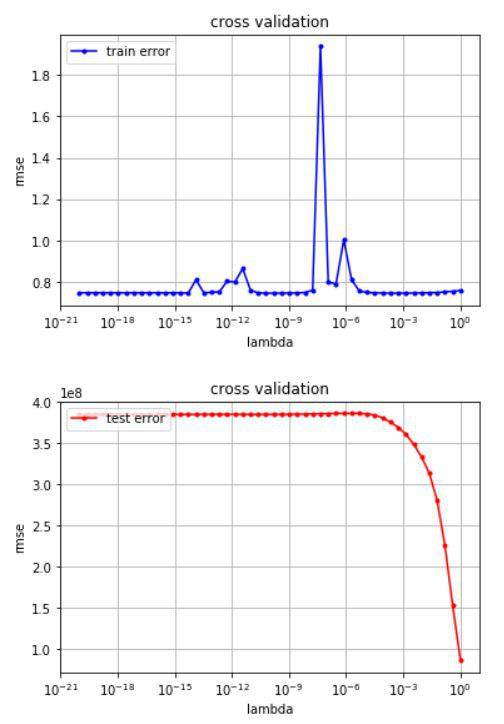
\includegraphics[width=.5\textwidth]{mse_cross_valid.jpg}
\caption{MSE of the train and test sets using cross validation on ridge regression}
\end{figure}
\section{Discussion}
Of course, as in every project, most of the stuff we tried didn't make it into the final thing, and as beginners in machine learning, we were quite disappointed to find out that the "silliest" method provided the best results for us. We wanted to apply Principal Component Analysis (PCA), which consists of working on the best eigenvectors from the dataset instead of the data in order to rid ourselves of the least valuable components, but as some people online said it, it improves results mostly when the amount of dimensions in our problem far outnumber the samples we have on hand. We tried using \texttt{least\_squares\_GD} and \texttt{least\_squares\_SGD}, but the score we got from there (about \textbf{0.685}) was not as good as what we have now, while with \texttt{logistic\_regression} and \texttt{reg\_logistic\_regression} would return \texttt{NaN}s. We also left out normalisation as we realized, to our great surprise, that it made us lose a lot of information, which ultimately hurt the results. The degrees and lambdas were of course all obtained by testing several possibilities to converge towards the best values before divergence.
\section{Conclusion}
Despite our disappointment about not being able to go beyond the methods that were proposed to us in the first place, we rejoice in the fact that we were able to make the best of them, with a respectable score of \textbf{0.81553}. We look forward to the next projects which will hopefully allow us to get a better understanding of more efficient methods, as we were often convinced that there was a better way of doing things that was lurking over us, yet we couldn't fully grasp it. It is remarkable to see how such a small program is able to give us such a glance into the world of particle physics, which we barely understand as of today. Even though we are fairly sure we do not have the best solution, getting to it was rather simple and the result has a quite high fidelity considering that more data would not necessarily bring a lot more to our results with the current methods.
\end{document}
